% Copyright 2019 the authors. All rights reserved.

% TODO:
% -

\documentclass[modern]{aastex62}

\usepackage{amsmath}

% typography
\setlength{\parindent}{1.\baselineskip}
\newcommand{\acronym}[1]{{\small{#1}}}
\newcommand{\package}[1]{\textsl{#1}}
\newcommand{\gaia}{\textsl{Gaia}}
\newcommand{\pans}{\textsl{Pan-STARRS}}
\newcommand{\DR}{\acronym{DR2}}
\newcommand{\msun}{\textrm{M}_\odot}
\newcommand{\kpc}{\textrm{kpc}}
\newcommand{\kms}{\ensuremath{\textrm{km}~\textrm{s}^{-1}}}
\newcommand{\bs}[1]{\boldsymbol{#1}}
\newcommand{\masyr}{\ensuremath{\textrm{mas}~\textrm{yr}^{-1}}}
\newcommand{\feh}{\ensuremath{[\textrm{Fe} / \textrm{H}]}}
\newcommand{\given}{\,|\,}

\newcommand{\sectionname}{Section}
\newcommand{\equationname}{Equation}
\renewcommand{\tablename}{Table}

\newcommand{\todo}[1]{{\color{red} TODO: #1}}

\newcommand{\changes}[1]{{\textbf{#1}}}
% \newcommand{\changes}[1]{{#1}}

% aastex parameters
% \received{not yet; THIS IS A DRAFT}
%\revised{not yet}
%\accepted{not yet}
% % Adds "Submitted to " the arguement.
% \submitjournal{ApJ}
\shorttitle{Stuff}
\shortauthors{People}

%@arxiver{}

\begin{document}\sloppy\sloppypar\raggedbottom\frenchspacing % trust me

\title{Palomar 5's biggest fan}

% \author[0000-0003-0872-7098]{Adrian~M.~Price-Whelan}
% \affiliation{Department of Astrophysical Sciences,
%              Princeton University, Princeton, NJ 08544, USA}
% \email{adrn@astro.princeton.edu}
% \correspondingauthor{Adrian M. Price-Whelan}

% \author[0000-0002-7846-9787]{Ana Bonaca}
% \affiliation{Harvard--Smithsonian Center for Astrophysics, Cambridge, MA 02138, USA}

\begin{abstract}\noindent % trust me
    Words!
\end{abstract}

\keywords{Galaxy: halo --- dark matter ---
          Galaxy: kinematics and dynamics}

\section{Introduction}
\label{sec:intro}


\section{Data}
\label{sec:data}

\begin{figure*}
\begin{center}
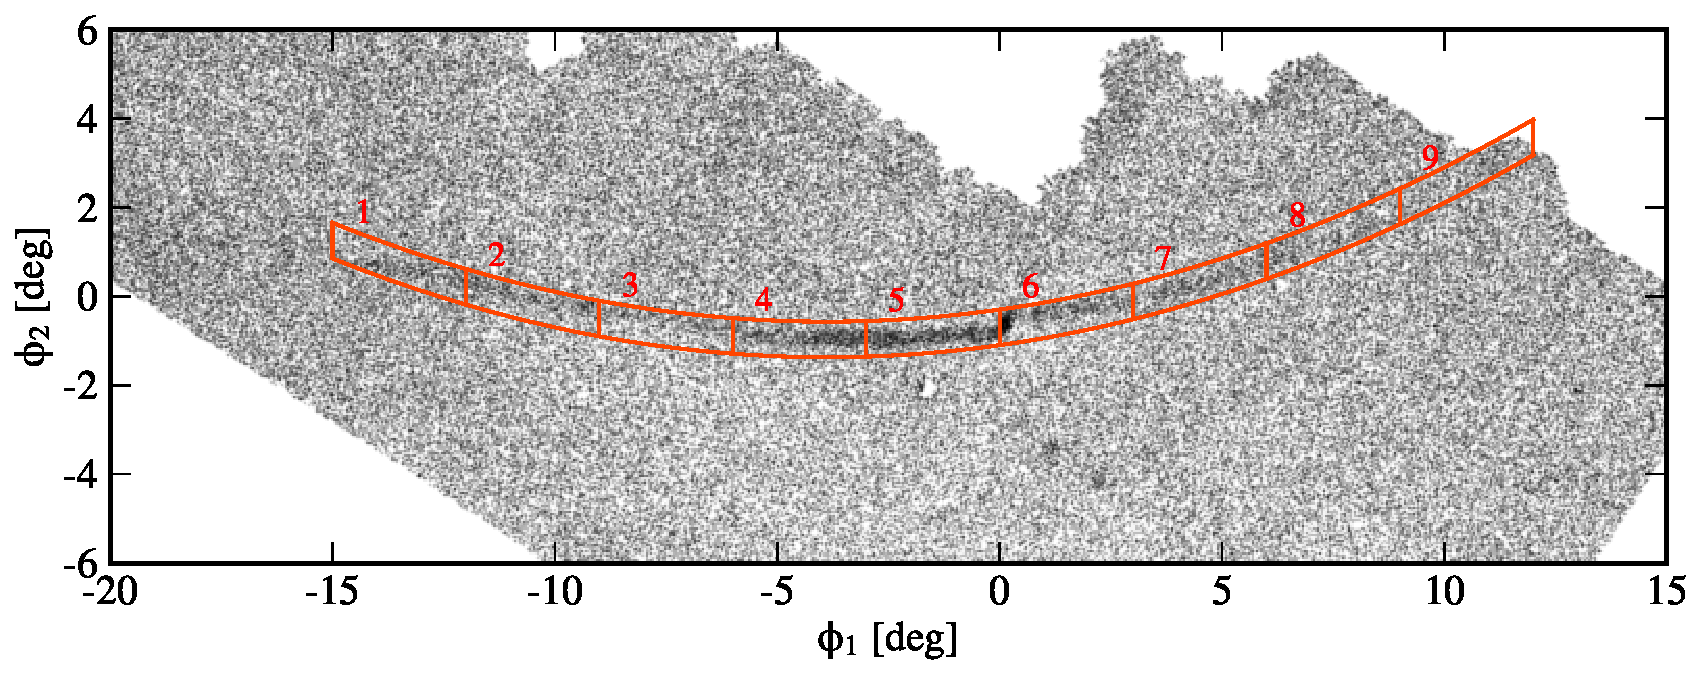
\includegraphics[width=0.8\textwidth]{fig1_a_map.pdf}
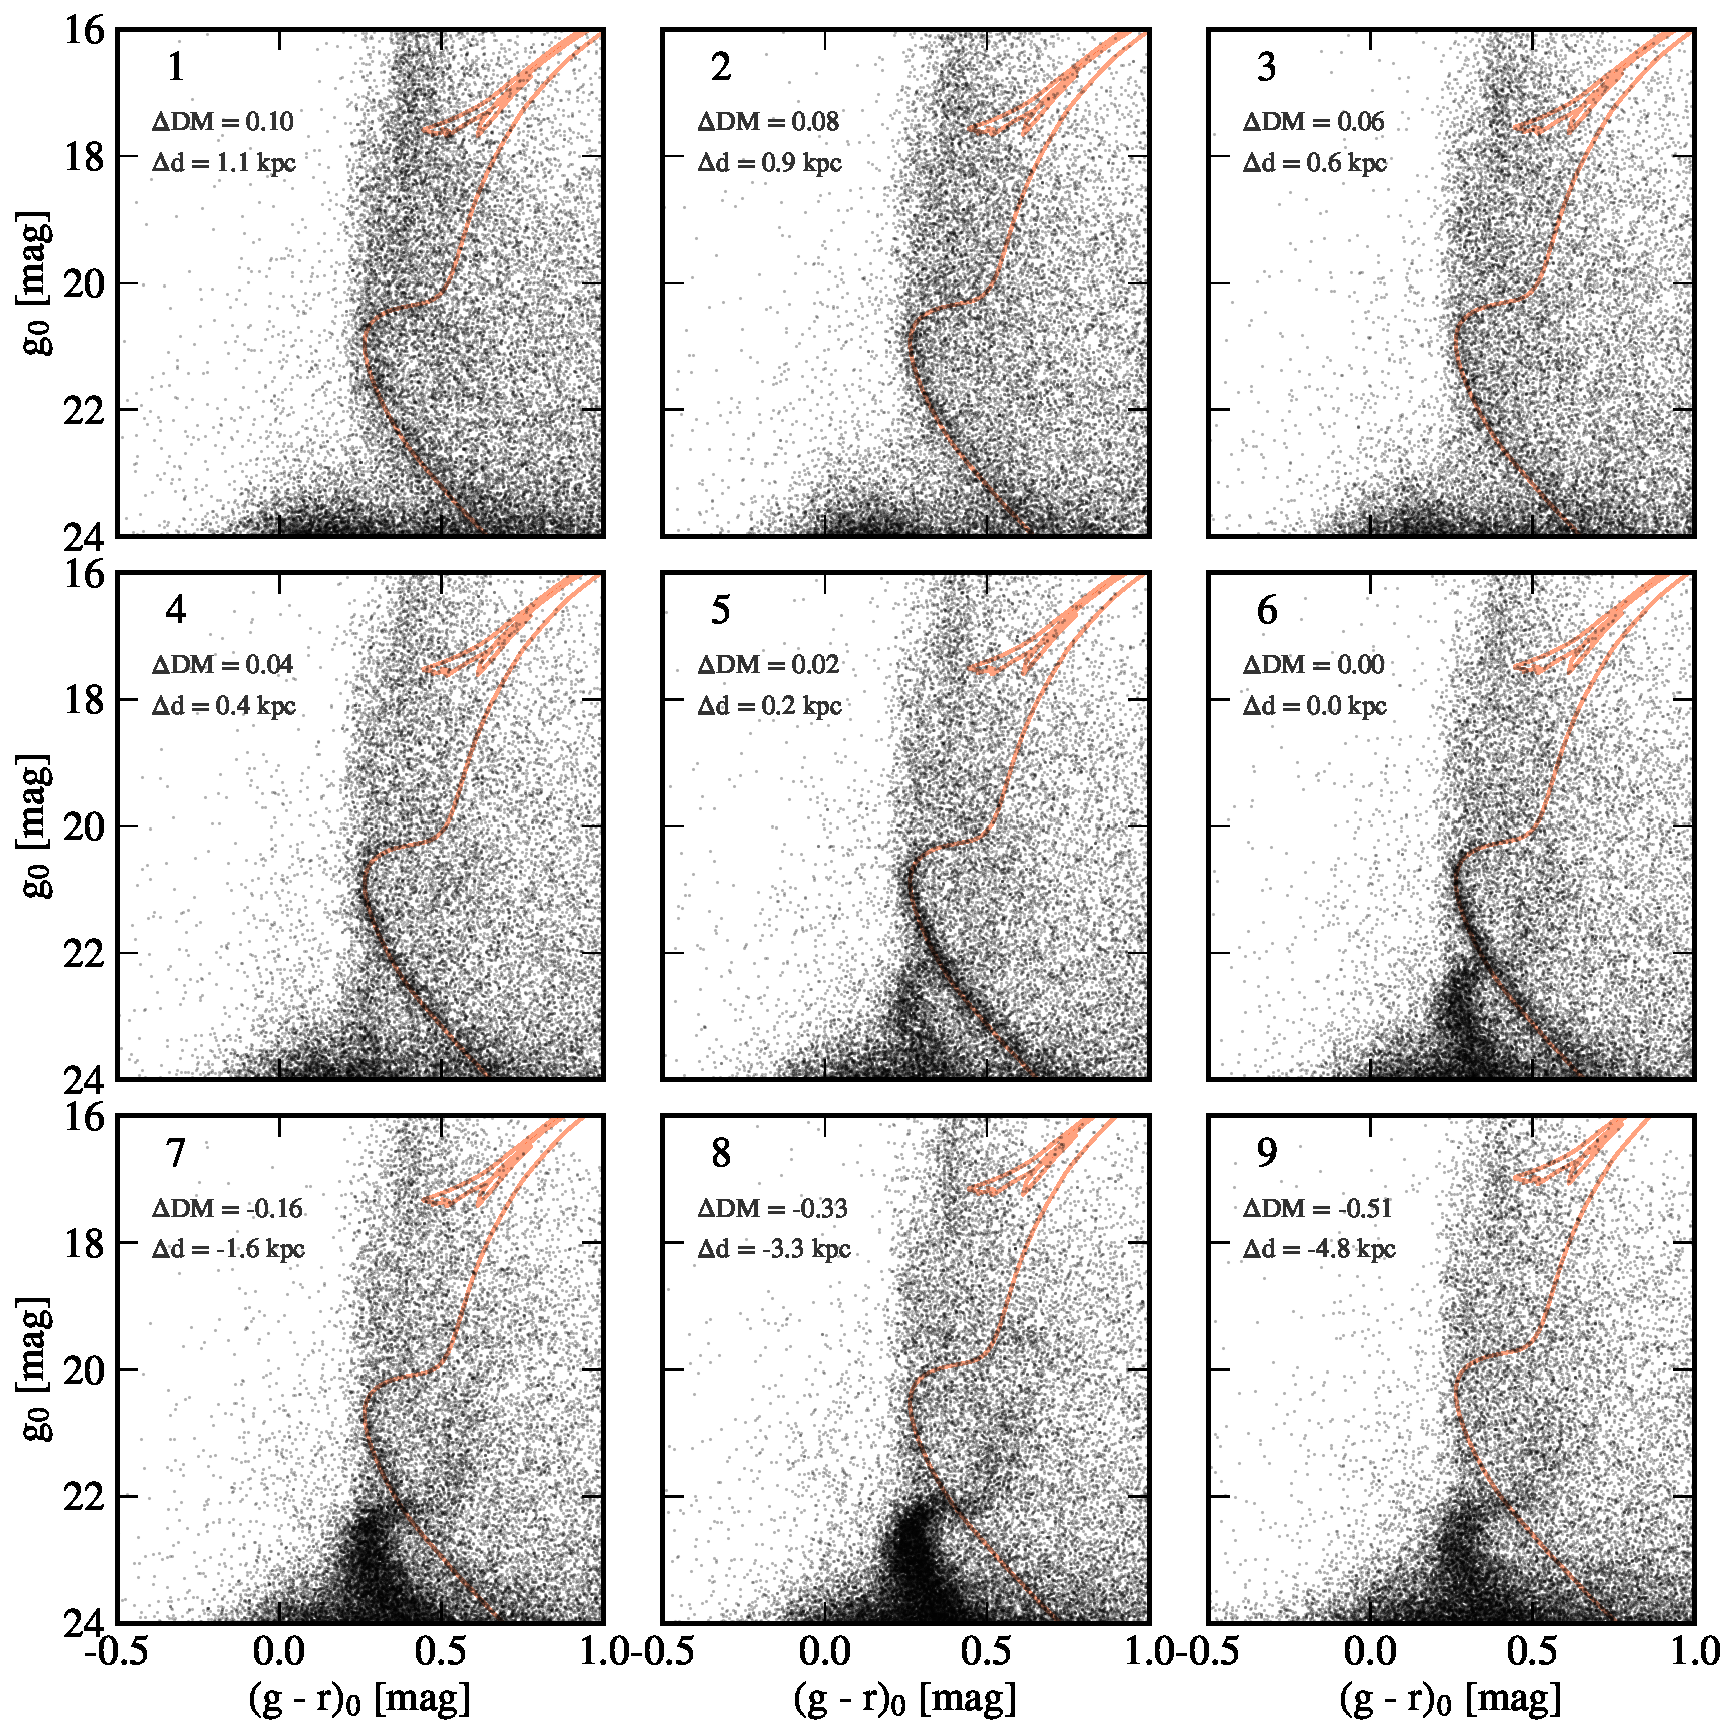
\includegraphics[width=0.8\textwidth]{fig1_b_cmds.pdf}
\end{center}
\caption{
% Best-fitting orbit of the Jhelum stellar stream in the disk plane (left) and perpendicular to the plane (right).
% Thicker portion of the line denotes the observed extent of the stream, while the insets present likely Jhelum members in these coordinates.
}
\label{fig:cmds}
\end{figure*}

\section{Simulations}
\label{sec:sim}
We run a suite of Pal 5 simulations to explore the mechanism leading the the observed morphology of the stream. In particular, we are interested reproducing the length asymmetry between the leading and trailing arm as well as the gap in the trailing arm and the ``fan" in the leading arm. In Section \ref{sec:potential}, we describe the potentials in which we simulate the evolution of Pal 5, and in Section \ref{sec:potential} we describe our suite of Pal 5 stream simulations. 

\subsection{Potential}
\label{sec:potential}
We simulate the evolution of Pal 5 in two types of potentials:

{\bf 1) NFW potential}: We use the {\small MWPotential2014} (\citealt{Bovy:2015}) consisting of a disk, bulge and halo. We use two different fattenings for the dark matter halo to illustrate Pal 5 on a regular as opposed to chaotic orbit.  

{\bf  2) Barred potential}: consisting af a disk, halo and bar with varying pattern speeds and bar masses.
Following \citet{wang:2012}, the bar potential is a basis-function (BFE) representation of a triaxial, exponential density profile. We include terms up to $n=9$, $l=19$ on the ``self-consistent field" BFE, as this yields a viable representation of the density of the bar (\citealt{banik:2019}). 

We explore a range of pattern speeds of the bar from $\Omega_b$ = (25 to 66) $\kms$ kpc$^{-1}$ in increments of 1 kpc$^{-1}$. Bars are not expected to extend beyond their co-rotation radius (\citealt{binney:2008}). Therefore given a pattern speed, we compute the co-rotation radius based on the mass profiles of the disk and halo and exponentially truncate our bar at this radius. If the scaling of the bar were left unaltered, this would significantly affect the gravitational  influence of the bar, as a slower bar would have its length underestimated and vice versa (\todo{subtily make the point that bovy and banik didn't do this?}).
Including the bar mass when calculating the co-rotation radius does not much affect the radius of co-rotation (see Figure). 

Additionally, we test two different bar masses, M$_{bar} = 5 \times 10^{9} \msun$ and M$_{bar} = 1 \times 10^{10} \msun$, respectively. 


\subsection{Stream modeling}
\label{sec:modeling}
For all simulations we assume a 6D phase space position of Pal 5 as: RA = 229.018 deg, Dec = - 0.24 deg, distance = 22.9 kpc, $v_r$ = -58.7 , pm$_{RA,cosdec}= -2.296$ mas and pm$_{Dec} = -2.257$ mas. We first transform Pal 5's 6D phase space position into a Galactocentric frame by assuming $v_{lsr} = (11.1, 24.0, 7.25) \kms$, 
$v_{circ} = 220  \kms$ and a distance from the Sun to the Galactic centre of 8.1 kpc. 

We first integrate the cluster backwards in time for 4 Gyr in steps of 0.5 Myr. Subsequently, simulate the evolution of Pal 5 using the ``particle-spray" stream modeling method developed by \citet{Fardal:2015}. We release two particles through each of the two Lagrange points every 10 Myr. We repeat this in first the NFW potential setting $q_z = 0.94$ (\citealt{Bovy:2016}) and subsequently in a flattened NFW potential ($q_z = 0.5$ to induce a chaotic orbit). 

Additionally, we simulate the evolution of Pal 5's stream in the barred potential




\section{Density model}
We first transform our  simulated Pal 5 data points to the tangent sky plane using a Zeanit (Lambert azimuthal) equal-area projection, such that we can define a Gaussian. We call these coordinates, $X$, $Y$.

We then fit a 3rd order polynomial to the leading and trailing arm separately, in this projected space. 

We place K nodes, k, equally in distance along the polynomial fits to the leading and trailing arm. 

At each node, k, along the polynomial we find the tangent/parallel unit vector,  $\hat{u}$, and the perpendicular normal unit vector, $\hat{v}$, to the stream. 

At each node, k, we define the co-variance matrix, $\tilde{C_k}$:

\begin{equation}
\tilde{C_k} = 
\begin{pmatrix}
    h^2 & 0  \\
    0 & S_k^2  \\
\end{pmatrix}
\end{equation}
where $h$ is bandwidth of the Gaussian components along the polynomial fit and $S_k$ is the  width of the Gaussians in the perpendicular (normal) direction of the stream at any node, k. 

We transform it from the space spanned by the $\hat{u}$,  $\hat{v}$ vectors to $X$, $Y$:
\begin{equation}
C_k = \rm{R} \tilde{C_k} \rm{R}^T
\end{equation}
where
\begin{equation}
\rm{R} = 
\begin{pmatrix}
    \rm{cos} \theta & - \rm{cos} \theta  \\
    \rm{cos} \theta & \rm{cos} \theta \\
\end{pmatrix}
\end{equation}
and  $\theta$ is the angle between the tangent sky plane and the unit vector, $\hat{u}$.

To compute our density model along the leading at trailing stream, for the K nodes, k, we define ln density  and sum over the K nodes:
\begin{equation}
\rm{ln} \sum ( \alpha_k \mathcal{N}\left(\mu_k, C_k\right))
\end{equation}
where $\mu_k$ denotes the location of each node, k, along the leading and trailing polynomial fits, respectively, $C_k$ is the covariance matrix, and $\alpha_k$ is the amplitude of the Gaussian (representing density at specific node, k). 

We then fit for the perpendicular width, $S_k$, to the stream (polynomial fits) and the amplitude of the Gaussians, $\alpha_k$, which represent the density along the stream. 

%Explain background model for data.

We compute the width and density of both or simulated Pal 5 streams and the DECaLS data fitting the above Gaussian mixture model. 

\section{Discussion}



\acknowledgements{
It is a pleasure to thank

% 
% This work has made use of data from the European Space Agency (ESA) mission {\it
% Gaia} (\url{https://www.cosmos.esa.int/gaia}), processed by the {\it Gaia} Data
% Processing and Analysis Consortium (DPAC,
% \url{https://www.cosmos.esa.int/web/gaia/dpac/consortium}). Funding for the DPAC
% has been provided by national institutions, in particular the institutions
% participating in the {\it Gaia} Multilateral Agreement.  This research was
% started at the NYC Gaia DR2 Workshop at the Center for Computational
% Astrophysics of the Flatiron Institute in 2018 April.
% 
% AB acknowledges generous support from the Institute for Theory and Computation
% at Harvard University.
% All code used in this work and all results are available at
% \url{https://github.com/adrn/GD1-DR2}.
}

\software{
    \package{Astropy} \citep{astropy, astropy:2018},
    \package{dustmaps}\footnote{\url{https://github.com/gregreen/dustmaps}},
    \package{gala} \citep{gala},
    \package{IPython} \citep{ipython},
    \package{matplotlib} \citep{mpl},
    \package{numpy} \citep{numpy},
    \package{scipy} \citep{scipy}
}

\bibliographystyle{aasjournal}
\bibliography{pal5fan}

\end{document}
